\chapter{System Design}
\label{chap:design}

\section{Assumptions}

Several assumptions are made in our design and implementation of VMMR system.

\begin{enumerate}
\item
	The input to the system are frontal images of vehicles.
\item
	Region of Interest (ROI) can be extracted from the input image based on a pre-labeled bounding box of number plate.
\item
	The true make and model label for any input image is one of the $27$ classes outlined in Section \ref{sec:dataset}.
\end{enumerate}

% \section{Graphical User Interface}

\section{Block Diagram}

A block diagram of our proposed VMMR system is presented in Figure \ref{fig:system}.

At the first stage, \textbf{Features Extraction Module} extracts features from the input image $I$ into a fix-length vector $F$. 
\textbf{Dimensionality Reduction Module} is optional and reduces the dimensionality of the high-dimensional vector $F$ into low-dimensional vector $F'$.
\textbf{Classification Module} is essentially a multi-class classifier that learns to assign incoming feature vectors to their corresponding true labels.


\begin{figure}
\centering
% 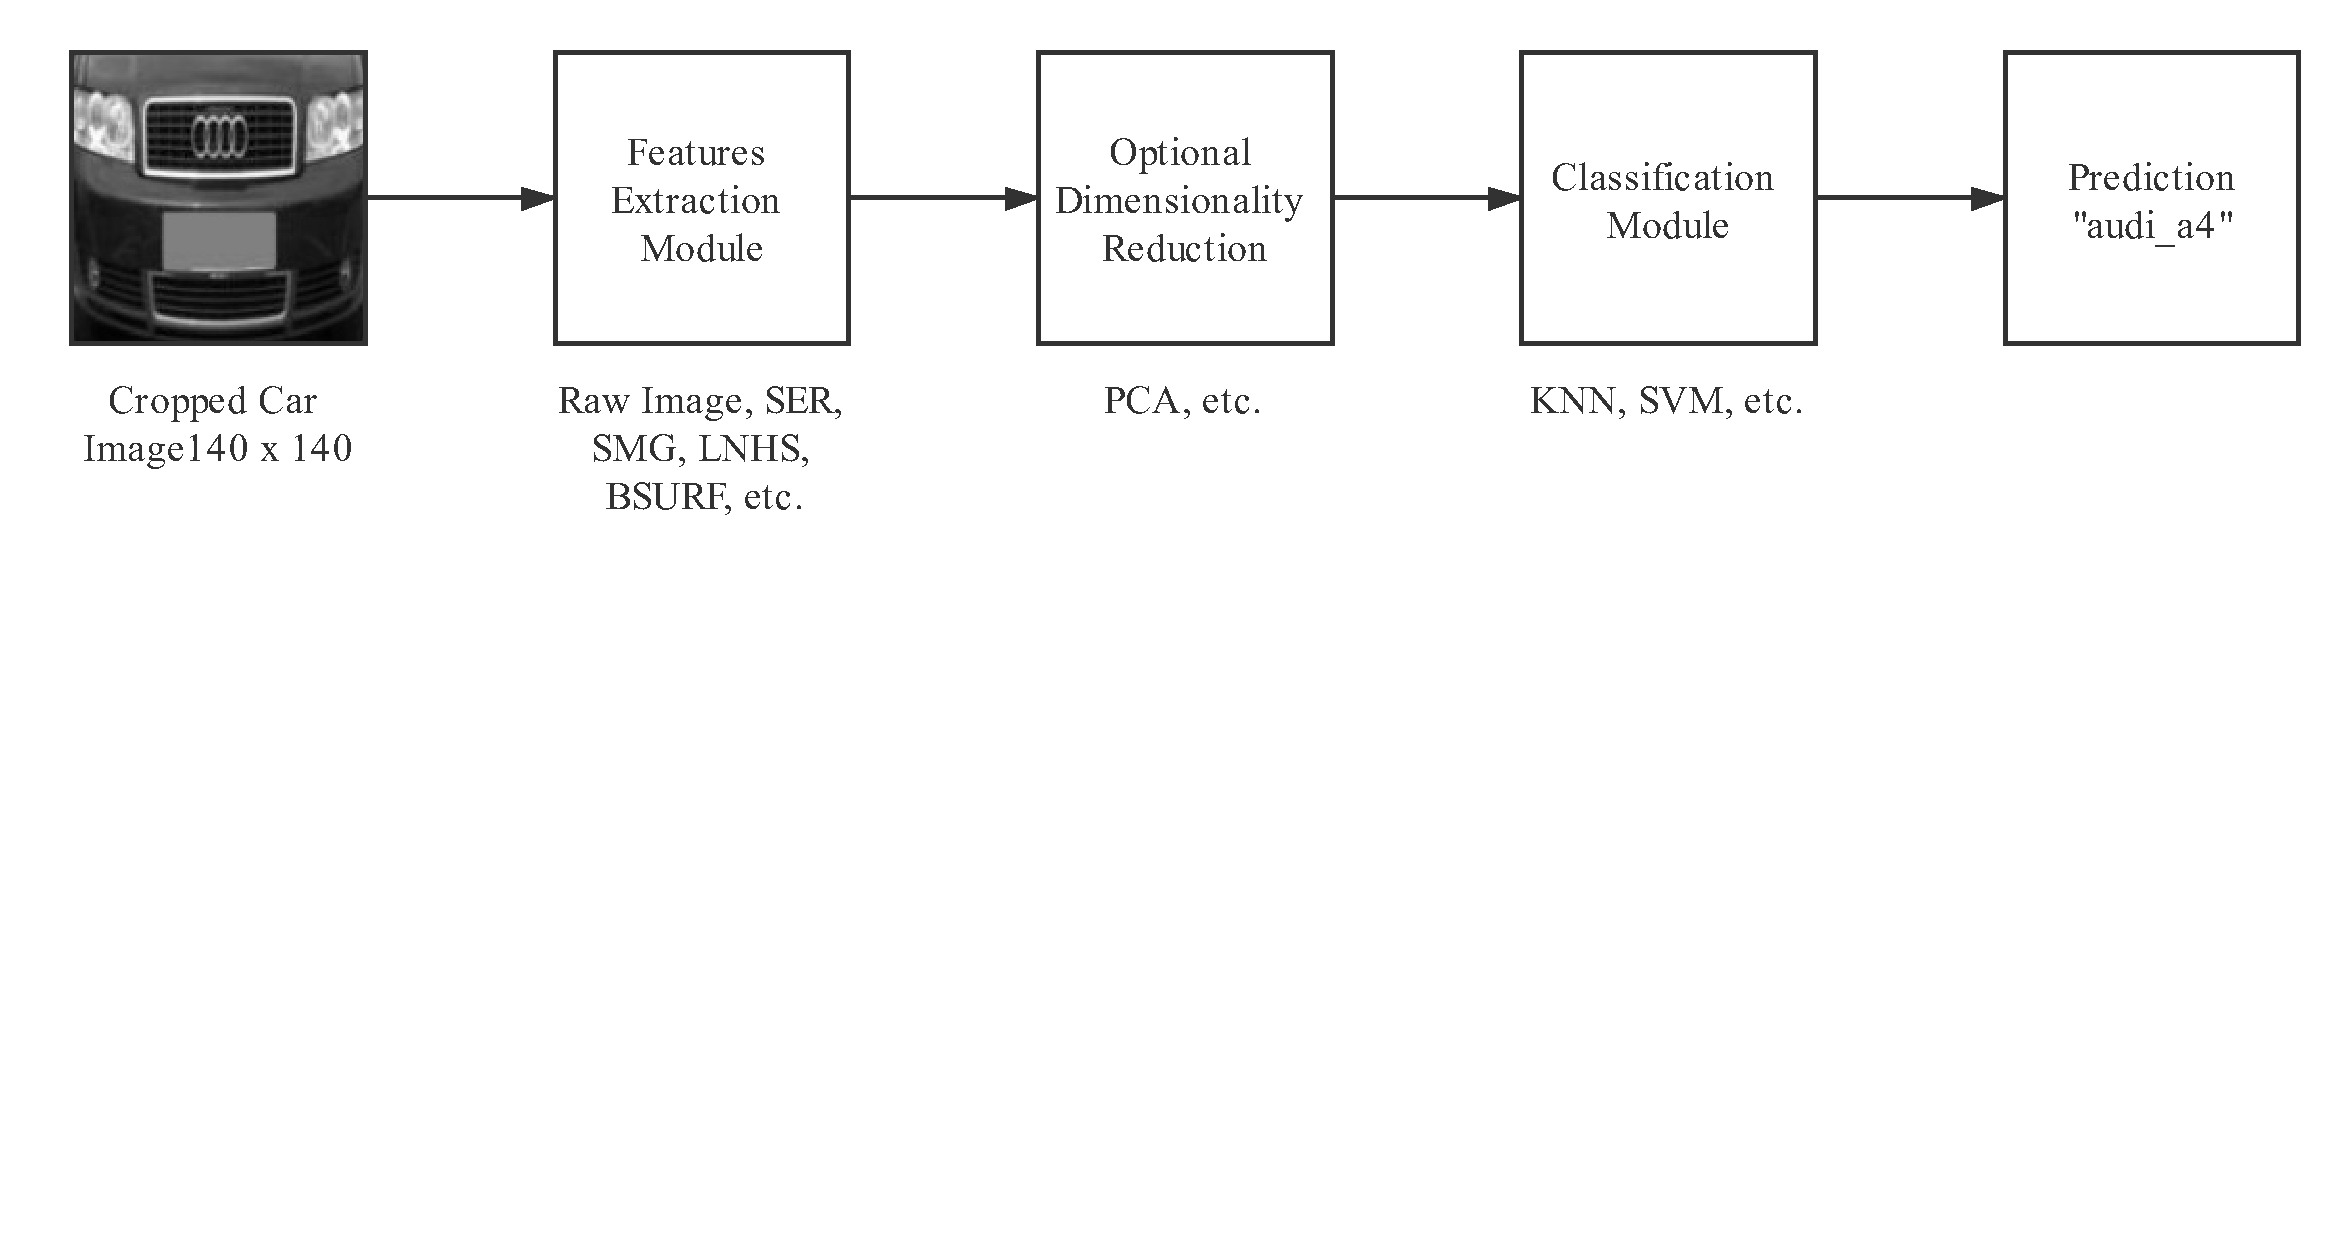
\includegraphics{system}
\caption{Block Diagram of Our Proposed VMMR System.}
\label{fig:system}
\end{figure}

\section{Features Extraction}

A variety of features are interchangeably computed in Features Extraction Module.
Among them, Raw Image, Sobel Edge Response (SER), Square Mapped Gradients (SMG) are parameter-free and first proposed to be used for VMMR by Petrovic and Cootes in \citep{petrovic2004analysis}.
Locally Normalised Harris Strengths (LNHS) is first proposed by Pearce and Pears in \citep{pearce2011automatic}.
Bag of Speeded Up Robust Features (BSURF) is first used by Siddiqui et al. for VMMR in \citep{siddiqui2016real}.

In Section \ref{sec:effects-fe}, the performance of the above features are compared and the effects of parameters of LNHS and BSURF on performance are examined.

\subsection{Raw Image}
Raw Image features are the image pixel values themselves. Hence, $F = I$.


\subsection{Sobel Edge Response (SER)}
SER (also named Sobel Gradient Map) is a map of weighted sum of pixels at 3-by-3 neighborhood.

\begin{equation}
S_{i,j} = \sum_{p=1}^3 \sum_{q=1}^3 W_{p,q} I_{i+p-2,j+q-2}
\end{equation}

where in y-direction, $W=W^y$ is specified as follows.

\begin{equation}
W_y = 
\begin{bmatrix}
  1&  2&  1 \\
  0&  0&  0 \\
  -1& -2& -1 
\end{bmatrix}
\label{equ:w}
\end{equation}

In x-direction, $W = W^{x} = W^{y} $.

The final feature vector $F$ is the concatanation of $S^x$ and $S^y$.

\begin{equation}
F = (S^x, S^y)
\end{equation}

\subsection{Square Mapped Gradients (SMG)}
SMG describes the parallel and diagonal components of change in Sobel Edge Response.
The parallel component $M^p$ and diagonal componet $M^d$ are computed as follows.

\begin{equation}
M^p_{i,j} = 
\begin{cases}
    0
    	,& \text{if } {S^x_{i,j}} =0 \text{ and } {S^y_{i,j}} =0\\
    \frac{{S^x_{i,j}}^2 - {S^y_{i,j}}^2}{{S^x_{i,j}}^2 + {S^y_{i,j}}^2}
    	,& \text{otherwise}
\end{cases}
\end{equation}

\begin{equation}
M^d_{i,j} = 
\begin{cases}
    0
    	,& \text{if } {S^x_{i,j}} =0 \text{ and } {S^y_{i,j}} =0\\
    \frac{2 \cdot {S^x_{i,j}}  {S^y_{i,j}}}{{S^x_{i,j}}^2 + {S^y_{i,j}}^2}
    	,& \text{otherwise}
\end{cases}
\end{equation}

The final feature vector $F$ is the concatanation of $M^p$ and $M^d$.

\begin{equation}
F = (M^p, M^d)
\end{equation}

\subsection{Locally Normalised Harris Strengths (LNHS)}
LNHS is a recurisve structure of Harris corner \citep{harris1988combined} features representaiton.
Given an image, Harris corner strengths $M = \{M_c\}$ are first computed following Noble's suggsted formulation \citep{noble1989descriptions}.

\begin{equation}
M_c = \frac{I_x^2 I_y^2 - (I_x I_y)^2}{I_x^2 + I_y^2}
\end{equation}

where $I_x$ and $I_y$ are smoothed image derivatives in x-direction and y-direction respectively.

Local Harris corner strengths $L$ are computed through recursively dividing the $M$ into quadrants and computing the sum of Harris corner strengths $M_c$ for each quadrant.
Local strengths are then normalised into a vector of LNHS through being devided by the sum of higher level strengths.

For example, for depth of $1$, $M$ is first divided into $4$ sub-matrices $M_{1}, M_{2}, \dots, M_{4}$.

\begin{equation}
M = 
\begin{bmatrix}
  M_{1}&  M_{2}\\
  M_{3}&  M_{4}\\
\end{bmatrix}
\end{equation}

The overall LNHS feature vector $F$ is equal to LNHS vector of depth $1$, $L_1$.

\begin{equation}
L_1 = \{\frac{sum(M_i)}{\sum_i sum(M_i)} | i \in \{1, 2, 3, 4\} \}
\end{equation}


For depth of $2$, the above $4$ sub-matrices $M_{1}, M_{2}, \dots, M_{4}$ are further divided into quadrants respectively.

\begin{equation}
M_{1} = 
\begin{bmatrix}
  M_{1,1}&  M_{1,2}\\
  M_{1,3}&  M_{1,4}\\
\end{bmatrix}
\end{equation}

LNHS vector of depth $2$ are computed through dividing the sum of each quadrant by the sum of its higher level quadrant.

\begin{equation}
L_2 = \{\frac{sum(M_{i,j})}{\sum_j sum(M_{i,j})} | i,j \in \{1, 2, 3, 4\}\}
\end{equation}

The overall LNHS feature vector $F$ is concantaion of LNHS vector of depth $1$ and $2$.

\begin{equation}
F = (L_1, L_2)
\end{equation}

Depth is the sole parameter in extracting LNHS features.

\subsection{Bag of Speeded Up Robust Features (BSURF)}
To compute a BSURF vector, SURF features \citep{bay2006surf} are first detected and extracted from the image.
A bag of visual words can be constructed by grouping all SURF feature descriptors from the training set into $T$ clusters using K-Means algorithm.

Given any image $I$, each SURF descriptor extracted can then be assigned to the nearest among the above $T$ clusters.
The BSURF feature vector $F$ for $I$ is a vector for visual words occurrences of fixed length $T$.

The number of clusters $T$ is the most important paramter in BSURF and is examined in our experiments.



\section{Dimensionality Reduction}
Features extracted from the images are usually correlated and can be reduced in dimensionality.
Such reduction speeds up the training and reduces the complexity of a classifier, which help prevents over-fitting issues.

\subsection{Principal Component Analysis (PCA)}
PCA maps high-dimensional data into a new low-dimensional coordinate system through Singular Value Decomposition (SVD).

Durining training, a high-dimensional matrix $X$ is formed, where each row is a feature vector $F$ extracted from a image in the training set.
SVM docomposes $X$ into a product of $3$ matrices.

\begin{equation}
X = U \Sigma W^T
\end{equation}

where $U$ is a m-by-m matrix, $\Sigma$ is a m-by-n diagonal matrix and $W^T$ is the transpose of $W$, a n-by-n matrix.

$X$ is then reduced in dimensionality to produce $X'$.

\begin{equation}
X' = X W_L
\end{equation}

where $W_L$ only preserves the first $L$ columns of $W$.

Likewise, for any 1-by-n feature vector $F$, a new vector $F'$ reduced in dimensionality can be derived.

\begin{equation}
F' = F W_L
\end{equation}

\section{Classification}
K-Nearest Neighbour (KNN) and Support Vector Machine (SVM) are used interchangeably in Classification Module. Their perforamnce are examined and compared in Section \ref{sec:effects-cls}.

\subsection{K-Nearest Neighbour (KNN)}
KNN is the simpest machine learning algorithm. 
A KNN classifier finds $K$-nearest neighbours for the input vector by Euclidean distance. 
The classifier then assigns each input vector to the most frequent class among its $K$-nearest neighbours.



\subsection{Support Vector Machine (SVM)}
In binary classification, SVM classifies each feature vector by learning to map in-coming features vectors into a separate space.
In multi-calss scnerario,  

